\documentclass[a4 paper]{article}
% Set target color model to RGB
\usepackage[inner=1.5cm,outer=1.5cm,top=2.5cm,bottom=2.5cm]{geometry}
\usepackage{setspace}
\usepackage[rgb]{xcolor}
\usepackage{verbatim}
\usepackage{amsgen,amsmath,amstext,amsbsy,amsopn,tikz,amssymb,tkz-linknodes}
\usepackage{fancyhdr}
\usepackage[colorlinks=true, urlcolor=blue,  linkcolor=blue, citecolor=blue]{hyperref}
\usepackage[colorinlistoftodos]{todonotes}
\usepackage{rotating}
%\usetikzlibrary{through,backgrounds}
\hypersetup{%
pdfauthor={Arman Shokrollahi},%
pdftitle={Homework},%
pdfkeywords={Tikz,latex,bootstrap,uncertaintes},%
pdfcreator={PDFLaTeX},%
pdfproducer={PDFLaTeX},%
}
%\usetikzlibrary{shadows}
\usepackage[francais]{babel}
\usepackage{booktabs}
\newcommand{\ra}[1]{\renewcommand{\arraystretch}{#1}}

      \newtheorem{thm}{Theorem}[section]
      \newtheorem{prop}[thm]{Proposition}
      \newtheorem{lem}[thm]{Lemma}
      \newtheorem{cor}[thm]{Corollary}
      \newtheorem{defn}[thm]{Definition}
      \newtheorem{rem}[thm]{Remark}
      \numberwithin{equation}{section}

\newcommand{\homework}[6]{
   \pagestyle{myheadings}
   \thispagestyle{plain}
   \newpage
   \setcounter{page}{1}
   \noindent
   \begin{center}
   \framebox{
      \vbox{\vspace{2mm}
    \hbox to 6.28in { {\bf\hfill} }
       \vspace{6mm}
       \hbox to 6.28in { {\Large \hfill #1 (#2)  \hfill} }
       \vspace{6mm}
       \hbox to 6.28in { {\it Instructor: #3 \hfill Student: #5} }
       %\hbox to 6.28in { {\it TA: #4  \hfill #6}}
      \vspace{2mm}}
   }
   \end{center}
   \markboth{#5 -- #1}{#5 -- #1}
   \vspace*{4mm}
}

\newcommand{\bbF}{\mathbb{F}}
\newcommand{\bbX}{\mathbb{X}}
\newcommand{\bI}{\mathbf{I}}
\newcommand{\bX}{\mathbf{X}}
\newcommand{\bY}{\mathbf{Y}}
\newcommand{\bepsilon}{\boldsymbol{\epsilon}}
\newcommand{\balpha}{\boldsymbol{\alpha}}
\newcommand{\bbeta}{\boldsymbol{\beta}}
\newcommand{\0}{\mathbf{0}}

\begin{document}
\homework{Actividad \#4}{Ajuste de Datos}{Carlos Liz\'arraga Celaya}{}{Antonio Cota Rodr\'iguez}{}

\section*{Introducci\'on}
\subsection*{Ajuste de Datos}
El ajuste de curvas consiste en encontrar una curva que contenga una serie de puntos y que posiblemente cumpla una serie de restricciones adicionales. Esta secci\'on es una introducci\'on tanto a la interpolaci\'on (cuando se espera un ajuste exacto a determinadas restricciones) y al ajuste de curvas o an\'alisis de regresi\'on (cuando se permite una aproximaci\'on).\\

El ajuste de curvas es un proceso mediante el cual, dado un conjunto de N pares de
puntos $(x_{i}, y_{i})$ (siendo $x$ la variable independente e $y$ la dependiente), se determina una
funci\'on matem\'atica $f(x)$ de tal manera que la suma de los cuadrados de la diferencia
entre la imagen real y la correspondiente obtenida mediante la función ajustada en cada
punto sea mínima: 

$$ \epsilon = min\left(\sum_{i=1}^{N}(y_{i}-f(x_{i}))^{2}\right) $$

Generalmente, se escoge una funci\'on gen\'erica $f(x)$ en funci\'on de uno o m\'as par\'ametros y se ajusta el valor de estos par\'ametros de la manera que se minimice el error
cuadr\'atico, $\epsilon$. La forma m\'as t\'ipica de esta funci\'on ajustada es la de un polinomio de grado $M$; obteni\'endose para $M = 1$ un ajuste lineal (o regresi\'on lineal), 

$$ f(x) = a_{0} + a_{1}x $$

para M = 2 un ajuste parabólico,

$$ f(x) = a_{0} + a_{1}x + a_{2}x^{2} $$ 

y as\'i sucesivamente.

\subsection*{Ajuste por m\'inimos cuadrados}

M\'inimos cuadrados es una t\'ecnica de an\'alisis num\'erico enmarcada dentro de la optimizaci\'on matem\'atica, en la que, dados un conjunto de pares ordenados —variable independiente, variable dependiente— y una familia de funciones, se intenta encontrar la funci\'on continua, dentro de dicha familia, que mejor se aproxime a los datos (un "mejor ajuste"), de acuerdo con el criterio de m\'inimo error cuadr\'atico.\\

Existen numerosas leyes f\'isicas en las que se sabe de antemano que dos magnitudes $x$
e $y$ se relacionan a trav\'es de una ecuaci\'on lineal

$$ y = {\bf{a}}x + {\bf{b}} $$

donde las constantes {\bf{b}} (ordenada en el origen) y {\bf{a}} (pendiente) dependen del tipo de sistema que se estudia y, a menudo, son los par\'ametros que se pretende encontrar. El m\'etodo de m\'inimos cuadrados determina los valores de los par\'ametros {\bf{a}} y {\bf{b}} de la recta que mejor se ajusta a los datos experimentales. Sin detallar el procedimiento, se dar\'a aqu\'i simplemente el resultado: 

$$ {\bf{a}} = \frac{n({\sum x_{i}y_{i}})-({\sum x_{i}})({\sum y_{i}})}{n(\sum x_{i}^{2})-({\sum x_{i}})^{2}} $$
\vspace*{0.2cm}
$$ {\bf{b}} = \frac{(\sum y_{i})-{\bf{a}}({\sum x_{i}})}{n} $$

donde $n$ es el n\'umero de medidas y $\Sigma$ representa la suma de todos los datos que se indican.

\newpage

\subsection*{Ajuste exponencial}

Cuando la curva de regresi\'on de $y$ sobre $x$ es exponencial, es decir para cualquier $x$ considerada, la media de la distribuci\'on est\'a dada por la siguiente ecuaci\'on predictora:

$$ y = Ab^{x} $$

Tomando el logaritmo en ambos miembros de la ecuaci\'on:

$$\log{y} = \log{A} + x\log{b} $$

Y se puede estimar ahora $\log{A}$ y $\log{b}$, y de ah\'i obtener $A$ y $b$ aplicando el m\'etodos de m\'inimos cuadrados.\\

Donde las constantes $A$ y $b$ quedan fijadas al resolver simult\'aneamente las ecuaciones:

$${\sum \log{y}} = N{\sum \log{A}} + {\log{b}}{\sum x}$$

$${\sum x}\log{y} = \log{A}{\sum x} + \log_{b}{\sum x^{2}} $$



\section*{Programas}
\subsection*{Temperatura de invierno en Nueva York (Ajuste lineal)}

El siguiente programa se utiliz\'o el ajuste lineal por el m\'etodos de m\'inimos cuadrados para las temperaturas medias registradas durante el invierno en la ciudad de Nueva York desde el a\~{n}o 1900 hasta 1999. El c\'odigo que es (en Python): 

\begin{verbatim}

import numpy as np
from scipy import optimize
import matplotlib.pyplot as plt


#Archivo de datos
data = np.loadtxt('NewYork.txt')

x=data[:,0].astype(np.int)
y=data[:,1].astype(np.float)

#Escala 
xn=np.linspace(1900,2000,2)

#Modulo polinomial
m, c = np.polyfit(x, y, 1)
#Aproximación de los coeficientes
yn = np.polyval([m, c], xn)

#Imprimir la grafica
plt.plot(x, y, 'or', label="Datos")
plt.plot(xn, yn, label="Ajuste")
plt.title('Temperatura en NewYork')
plt.legend()
plt.show()

\end{verbatim}

\newpage
La gr\'afica ya ajustada es la siguiente:

\begin{figure}[!ht]
  \centering
      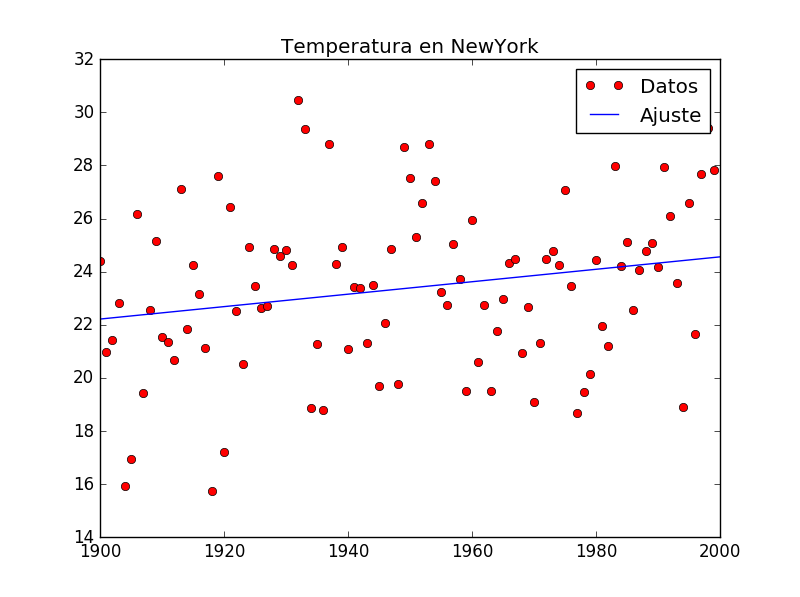
\includegraphics[width=8cm, height=6cm]{Ajuste_Lineal.png}
  \caption{Ajuste lineal}
\end{figure}

\section*{Presi\'on atmosf\'erica vs. altitud (Ajuste exponencial)}

En esta secci\'on se muestra un c\'odigo para Python, en el cual se observa una relaci\'on entre la presi\'on atmosf\'erica y la altitud, estos datos obtenidos del art\'iculo {\it{Arguado E and Burt JE (1999), Understanding Weather and Climate; Prentice Hall, Saddle River, New Jersey.}}. El c\'odigo es el siguiente:

\begin{verbatim}
import numpy as np
from scipy import optimize
import matplotlib.pyplot as plt

#Archivo de datos
data1=np.loadtxt('Presión_Altitud.txt')

x1=data1[:,0].astype(np.int)
y1=data1[:,1].astype(np.float)


#Definiendo la funcion
def f(x,u,v,w):
    return u*np.exp(-v*x) + w
    
#Opitimizar la curva    
popt, pcov = optimize.curve_fit(f, x1, y1)


    
xm=np.linspace(-0,50,1000)

plt.plot(x1, y1, 'or', label="Datos")
plt.plot(xm,f(xm,*popt), label="Ajuste")

#Imprimir la grafica
plt.title('Presión-Altitud')
plt.legend()
plt.xlabel("Altitud")
plt.ylabel("Presión")
plt.show()
\end{verbatim}

\newpage
con su respectiva gr\'afica ajustada:

\begin{figure}[!ht]
  \centering
      \includegraphics[width=8cm, height=6cm]{Presi_n_Altitud.png}
  \caption{Ajuste exponencial}
\end{figure}

\section*{Conclusi\'on}

En esta pr\'actica aprendimos una potente herramienta computacional para el manejo y visualización de datos que nos ser\'a de gran ayuda durante nuestra vida académica como fuera de ella.



\end{document}